\chapter{Optimizing network-utilization by balancing workload}
\label{chap:balancing}

The last chapter brings an overview of different notations, algorithms and techniques.
In this chapter, all these instruments are combined to a chain for distributing routes more evenly, that are preferred by routing-algorithms like \textit{Dijkstra}.

For a given \gls{acr:sdpair} and a graph $G$ of $d$-dimensional edge-weights, a path should be found through an algorithm, that implicitly tends to distribute found paths over the network while keeping the paths' costs sufficiently near every cost-dimension's optimum.
To achieve this, a preprocessing-phase called \textit{balancing} analyzes the graph $G$ and computes a new metric for every edge.
With this metric, routing-algorithms like \textit{Dijkstra} \todo{TODO Check if \textit{Dijkstra} really improves distribution or \textit{cyclops} has to be used.} (with \textit{personalized routing}) and \textit{cyclops} can compute paths as usual.

This \textit{balancing} is depicted in figure~\ref{fig:balancing}.

\begin{figure}
    \centering
    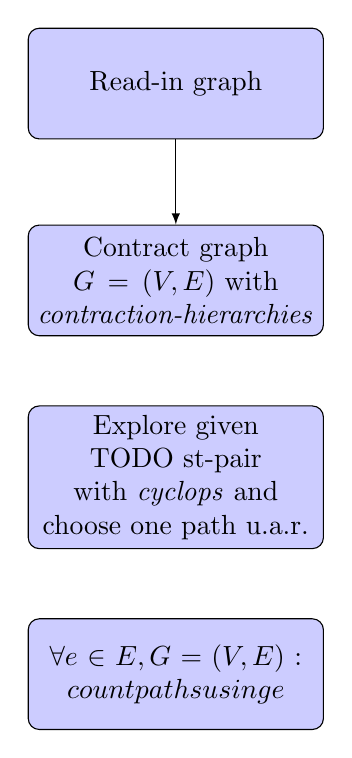
\begin{tikzpicture}[auto, rounded corners=0, node distance = 3cm, x=1cm, y=1cm] {%
    % style

    % draw
    % Draw borders

    % text badly centered
    % better use 'align=flush center'

    \tikzstyle{decision} = [%
        diamond,
        draw,
        fill = blue!20,
        text width = 4.5em,
        align = flush center,
        node distance = 3cm,
        inner sep = 0pt
    ]
    \tikzstyle{block} = [%
        rectangle,
        draw,
        fill = blue!20,
        text width = 10em,
        text centered,
        rounded corners,
        node distance = 2.5cm,
        minimum height = 4em
    ]
    \tikzstyle{cloud} = [%
        draw,
        ellipse,
        fill = red!20,
        node distance = 3cm,
        minimum height = 2em
    ]

    % arrow-styles
    % https://tex.stackexchange.com/questions/5461/is-it-possible-to-change-the-size-of-an-arrowhead-in-tikz-pgf
    \tikzstyle{line} = [draw, -latex]

    % Place nodes

    \node [block] (read-in_graph) {Read-in graph};
    \node [block, below of = read-in_graph] (contract_graph) {Contract graph $G=(V,E)$ with \textit{contraction-hierarchies}};
    \node [block, below of = contract_graph] (exploration) {Explore given TODO st-pair with \textit{cyclops} and choose one path u.a.r.};
    \node [block, below of = exploration] (analyzation) {$\forall e \in E, G = (V, E): count paths using e$};

    % Draw lines

    \path [line] (read-in_graph) -- (contract_graph);

    % \node [block] (init) {initialize model};
    % \node [cloud, left of=init] (expert) {expert};
    % \node [cloud, right of=init] (system) {system};

    % \node [block, below of=init] (identify) {identify candidate models};

    % \node [block, below of=identify] (evaluate) {evaluate candidate models};
    % \node [block, left of=evaluate, node distance=3cm] (update) {update model};

    % \node [decision, below of=evaluate] (decide) {is best candidate better?};

    % \node [block, below of=decide, node distance=3cm] (stop) {stop};

    % % Draw edges

    % \path [line] (init) -- (identify);
    % \path [line] (identify) -- (evaluate);
    % \path [line] (evaluate) -- (decide);
    % \path [line] (decide) -- node {no} (stop);

    % \path [line] (update) |- (identify);
    % \path [line] (decide) -| node [near start] {yes} (update);

    % \path [line,dashed] (expert) -- (init);
    % \path [line,dashed] (system) -- (init);
    % \path [line,dashed] (system) |- (evaluate);
} \end{tikzpicture}
    \caption[Overview of balancing a graph]{%
        This flow shows the balancer, that analyzes a given graph $G$.
        Actions are rectangular, data is elliptical.
        A metric is created and updated, that distributes upcoming workload (like during rush-hour) more evenly over the graph.
        \label{fig:balancing}
    }
\end{figure}

\todo{TODO Routes within a certain tolerance of the best possible cost (per metric, e.g. duration must be not worse than $25~\%$ \todo{tolerance should match the resulting plots}) are randomly chosen from \textit{cyclops}.}

\section{Implementation}
\label{chap:balancing:implementation}

\todo{TODO}

    \subsection{Accessing the graph-structure}

    \todo{TODO add some text here}

    \subsection{Configs}

% - indices -> boost for performance while staying dynamic
% - Dijkstra, no A* because multiple metrics vs heuristic
% Mainly describing
% - choose alternative routes -> better total workload in street-network
% - both approaches: multiple runs (explicit euler) vs multiple metrics
% - highlights, what was difficult/much work? -> repo-link
% - implementation -> sub-chapter of chapter 3
% - normalization of all metrics -> comparability between different graphs